\chapter{Einleitung}
\label{chap:einleitung} Die Computertomografie (CT) hat die Medizintechnik revolutioniert
und ist bis heute eines der wichtigsten Methoden für die Bildanalyse. Sie ist
eine der führenden Erweiterungen der klassischen Röntgentechnik. Für die Entwicklung
dieser Technologie wurden Godfrey Newbold Hounsfield und Allan McLeod Cormack im
Jahre 1979 mit dem Nobelpreis für Medizin ausgezeichnet \citep[Seite12]{handels2000}.

\begin{minipage}{0.40\textwidth}
	Die Computertomografie wird in den verschiedensten Bereichen und im wahrsten Sinne
	des Wortes von Kopf bis Fuß eingesetzt. So kommt es, dass auch im Dentalbereich
	CT Aufnahmen von größter Wichtigkeit sind. Abbildung
	\ref{fig:ct_aufnahme_eines_zahns} zeigt eine solche CT-Aufnahem. Eine konkrete
	Anwendung in diesem Kontext ist die Zahnkaries Forschung der Poliklinik für Zahnerhaltung
	und Parodontologie des LMU- Klinikums München.
\end{minipage}
\hfill
\begin{minipage}{0.50\textwidth}
	\centering
	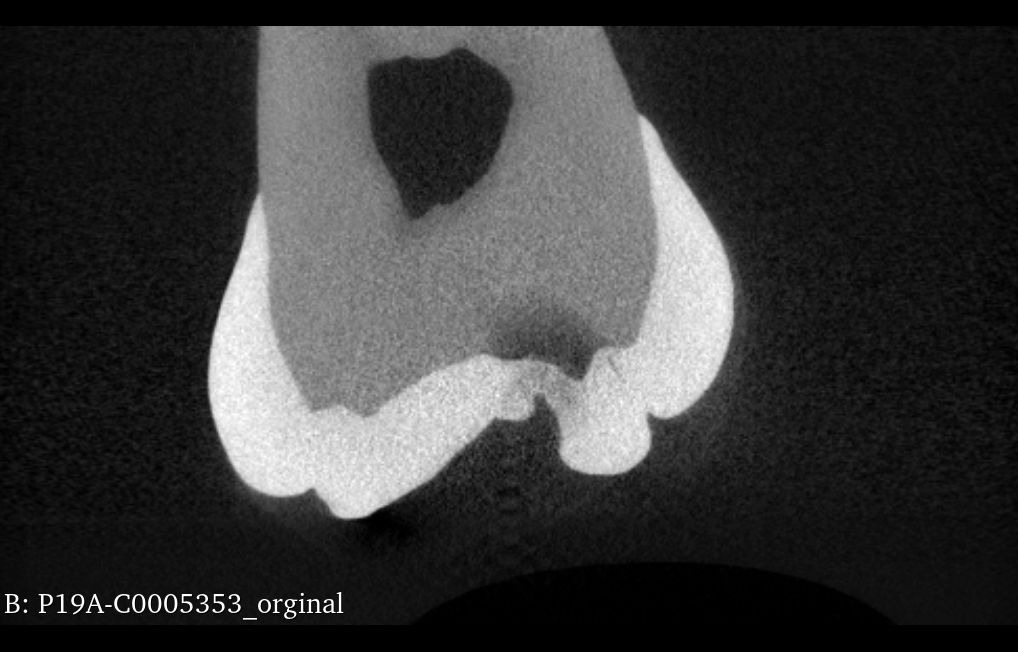
\includegraphics[scale=0.2, width=\textwidth]{img/micro_ct_orginal.jpg}
	\captionof{figure}{CT-Aufnahme eines Zahns \\ Quelle \citep{poliklinikLMU}} \label{fig:ct_aufnahme_eines_zahns}
\end{minipage}

Die vorliegende Arbeit soll genau diese Forschung unterstützen. In welchem Umfang
und zu welchem Grund ist in den folgenden Abschnitten beschrieben.
% ---------------------------------------------------------------------------------------

\section{Ziel der Arbeit}
\label{sec:ziel_der_arbeit} Diese Arbeit beschreibt eine Technik, mit der
dreidimensionale Micro-CT Bilder zur Untersuchung zahnmedizinischen Strukturen
automatisch mittels der Software \textit{3D Slicer} segmentiert und analysiert werden
können. Die algorithmische Formulierung einer konkreten Segmentierung ist
bereits vorhanden und prototypisch implementiert. Dieser Algorithmus muss jedoch
umständlich über ein Kommando im Terminal ausgeführt werden, was die
Benutzerfreundlichkeit deutlich beeinträchtigt. Ziel dieser Arbeit ist es nun das
bereits implementiert Verfahren automatisiert über ein interaktives User Interface
(UI) zur Verfügung zu stellen. Dabei soll auf etablierte und vertraute Lösungen
zurückgegriffen werden.

Es stellt sich nun die Frage, zu welchem Zweck eine automatische und interaktive
Segmentierung überhaupt notwendig ist. Für die Zahnklinik an der LMU in München
gibt es hierfür viele Gründe. Über den wichtigsten gibt das nächste Kapitel Aufschluss.
% ---------------------------------------------------------------------------------------

\section{Relevanz der Arbeit}
\label{sec:relevanz_der_arbeit} Der wohl relevanteste Punkt dieser Arbeit ist,
dass Ärzte reine Anwender und keine Entwickler von Software sind. Darüber hinaus
verfolgt die Parodontologie der LMU in München einen sehr interessanten Forschungsansatz,
welche eine Segmentbetrachtung der CTs unumgänglich macht.

Über viele Jahre hinweg wurden in der Zahnklinik sehr viel Bilddaten von Zähnen
gesammelt, die aufgrund von Zahnkaries entfernt wurden. Hierbei wurden Aufnahmen
der unterschiedlichsten Arten gemacht. Darunter fallen zum Beispiel einfache Bilddateien,
Infrarotbilder und die für diese Arbeit so relevanten dreidimensionalen Micro-CT
Aufnahmen. Dieser große Schatz an Bildmaterial soll verwendet werden, um in
ferner Zukunft ein neuronales Netzwerk zu trainieren, welches statistische Aussagen
über das Verhalten von Karies treffen kann. Jedoch gibt es hier ein Problem, bei
dem das Ergebnis dieser Arbeit Unterstützen kann.

Karies auf CT-Bildern zu lokalisieren ist nicht trivial. Er ist ohne weitere
Bearbeitung des Bildes nur sehr schwer auf eine Stelle einzugrenzen. So kommt es
vor, dass drei verschiedene Ärzte auf dem selben Micro-CT Bild drei
unterschiedliche Stellen mit Karies identifizieren. Eine Segmentierung des dreidimensionalen
CTs kann hier Wunder wirken lassen. Durch die Aufteilung des Micro-CTs in seine
zwei Zahnhauptsubstanzen, kann in das innere der Zähne geblickt werden, was die Lokalisierung
kariöser Stellen deutlich vereinfacht.

Mit dieser klaren und einduetigen identifizierung von Karies, sind die
Ergebnisse, die ein neuronales Netzer generieren würde viel genauer und brauchbarer.
Konkret wird mit einer automatischen Segmentierung ein \textit{Ground Trueth} gewonnen,
der eine eindeutige Basiswahrheit liefert.

Hierbe sei gesagt das diese Anwendung nur ein von vielen Möglichkeiten ist. Konkrete
Daten über die Ausbreitung einer Krankheit im Menschlichen Körper zu besitzten kann
in den verschiedensten Fällen und Institutionen von größtem Nutzen sein. So
zeigen es auch \citet{de20083d} in ihrem Paper. Dieses Argument stand dehmnach
auch für diese Arbeit bereits zu Beginn im Mittelpunkt und bildet somit den
Fokus der Untersuchung, welcher im Nachfolgenden Kapitel näher beleuchtet werden
soll.
% ---------------------------------------------------------------------------------------

\section{Fokus der Arbeit}
\label{sec:fokus_der-arbeit} Für eine automatische Segmentierung von Micro-CT Bildern
gibt es einige Softwarelösungen am Markt, die alle eine gut optionen sind. Dieser
Arbeit setzt den Fokus auf die Open Sorce Plattform \textit{3D Slicer}, da diese ohnehin
bereits eine breite Anwendung in der Zahnklinik in München findet. Durch die
Modul und Plugin Infrastruktur dieser Plattform kann die Softwar auch anderen Institutionen
bereitgestellt werden. Hierzu muss diese einfach als \textit{3D Slicer Extetion}
bereitgestellt werden. \textit{3DSlicer} bietet einen Extension Manager, der
ähnlich wie ein App Store betrachtet werden kann. So bleibt die vorerst konkret entwickelte
Software nicht nur einer Einrichtung vorbehalten.

Diese Arbeit setzt so den Fokus auf die Extention von \textit{3D Slicer} um so
eine automatische und interkative Schnittstelle zu gewähren. Die Optimierung des
bereits bestehenden Verfahrens wird nicht thematisiert.

Mit dieser Umfang, der Motiavtion und dem gesetzten Fokus, ergibt sich für dies Arbeit
eine konkrete Struktur die nun kurz erläutert werden soll.
% ---------------------------------------------------------------------------------------

\section{Aufbau der Arbeit}
\label{sec:aufbau_der_arbeit} Die Arbeit ist in sieben Kapitel unterteilt. Nach
der Einführung in Kapitel \ref{chap:einleitung}, in der die Relevanz und der Fokus
beschrieben werden, werden in Kapitel \ref{chap:theoretische_grundlagen} die
theoretischen und technischen Grundlagen behandelt, welche zum Verstehen der Ergebnisse
essenziell sind. Als Ergebnis der theoretischen Grundlagen bildet das Kapitel
\ref{chap:fragestellung} eine konkrete Forschungsfrage. Während sich Kapitel \ref{chap:methodik}
darum kümmert mit welchen Methodiken und Lösungsansätzen an die Forschungsfrage herrangegangen
wird, erläutert das Kapitel \ref{chap:ergebnisse} was die konkreten Ergebnisse
der Arbeit sind. In Kapitel \ref{chap:diskussion} erfolgt eine kritische Diskussio
der Resultate einschließich möglicher Limitationen. Das Abschließende Kapitel\ref{chap:schlussfolgerung}
fasst die wichtigsten Erkenntnisse zusammen und gibt einen Ausblick auf zukünftige
Forschungsfragen.

Die theoretischen Grundlagen die wie beschrieben nach der Einleitung folgen,
sind zentral für das Versetehen der Fragestellung und der methodischen
Ausarbeitung.
% ---------------------------------------------------------------------------------------